\documentclass{article} % For LaTeX2e
\usepackage{nips13submit_e,times}
\usepackage{hyperref}
\usepackage{url}
\usepackage{authblk}
\usepackage{graphicx}
\usepackage[numbers]{natbib}
\usepackage{amsmath}

%\documentstyle[nips13submit_09,times,art10]{article} % For LaTeX 2.09

\begin{document}

\author{Bai, Min \texttt{mbai@cs.toronto.edu}}
\author{Loyzer, Mark \texttt{loyzer@cs.toronto.edu}}
\affil{Department of Computer Science
University of Toronto
Toronto, Ontario, Canada}

\newcommand{\fix}{\marginpar{FIX}}
\newcommand{\new}{\marginpar{NEW}}

\nipsfinalcopy % Uncomment for camera-ready version

\begin{abstract}
text here
\end{abstract}

\section{Introduction}
This project focuses on classifying digits from street view images.  We use the Street View House numbers dataset from \cite{svhn}. All images have a fixed 32x32 resolution with character-level ground truth labels. For each example, the labelled character is centered at the image. Since this is a digit recognition task there are ten classes in total.

The data is collected from street-view images, thus there exist vast intra-class variations. To generate competitive performance, we have considered a variety of classification techniques exploiting feature representations that are robust to intra-class variations. We attempt both hand-crafted and learned features as well as raw pixel data as the purpose of this project is to investigate different machine learning techniques and so knowing the pitfalls and prevalences of each technique.

\section{Convolutional Neural Networks}

\subsection{Setup}

The first method we explored is the convolutional neural networks technique. The architectures explored are based on a 2012 CVPR paper \cite{lecun2012}, as well as the tutorials provided by Google in their Tensorflow tutorials \cite{googletensorflow}. 

The basic structure of the network consists of several convolution layers followed by several fully connected layers, which finally finally feed to a 10 unit softmax output. The details of these layers is discussed in the following sections. 

\subsubsection{Convolution Layer}

The standard convolution layer consists of a 2 dimensional patch of size 5x5. The layer takes in M input feature channels, and produces N output feature channels by through parallelism. The convolution operation is described by the following equation. 

\begin{gather}
{h_{i,j,n}}^l = \sigma(\sum_{e=1}^{M}{\sum_{a=-2}^{2}{\sum_{b=-2}^{2} w_{a,b,m,n}h_{(i+a),(i+b),m}^{l-1}} + b_n}) \\
\sigma(x) = \text{max}\{0, x\}
\end{gather}

where ${h_{i,j,n}}^l$ is the (i,j)-th indexed output in the l-th layer in channel n, while $w_{a,b,m,n}$ is a weight in the convolution layer, and $b_n$ the bias value for the n-th output layer. 

\subsubsection{Local Response Normalization Layer}

The local response normalization layer is akin to a image whitening, whereby the input to the next layer is rescaled so that the nearby neurons receive input of roughly the same size. This can theoretically improve training performance. 

\subsubsection{Pooling Layer} 

Max pooling is used to reduce the size of the image, and to provide some shift invariance. Since we are only attempting to detect one number in the input image, the use of max pooling allows us to find the area with the maximum response. The pooling function operates over a 2x2 square, and returns the maximum value among the 4 values in the square. Moreover, the pooling scheme has a stride size of 2, effectively having no overlap. It has been shown that pooling can contribute significantly to object recognition based on convolutional neural networks \cite{pooling}, and it is hoped that it will be useful for digit recognition as well. 

\subsubsection{Fully Connected Layer}

The fully connected layers are used at the output of the neural network. This is the standard neuron, with every neuron connected to all neurons in the preceding and following layer. The model is as follows:

\begin{gather}
{h_{j}}^l = \sigma({w_{i,j}}^{l} {h_{i}}^{l-1} + {b_j}^l) 
\end{gather}

\subsubsection{Implementation and Training}

Various configurations using the preceding network layers are instantiated using the Google TensorFlow package. The network is then optimized using the built in AdamOptimizer, with the cross entropy as the cost function to be minimized:

\begin{gather}
J(w) = - \sum_{i}{\sum_{k=0}^{9}{t^{(i)}_k}log(y_k(x^{(i)}))}
\end{gather}

where t are the one-hot targets, and y is the the output vector of the final multi-class softmax function. 

Mini-batch training is used to train the neural networks, with 50 input samples per batch. These mini-batches are selected at random with replacement from the sample set. Both the training and extra-training input images from the SVHN website are used, for a total of 604388 training samples. Because of the large quantity of test data available (26032 samples, which is on average 2600 samples per digit), we decided to use 10000 of these for the validation set, and the remaining 16032 for the test set to obtain an unbiased estimate of the performance of our implementation.

Through experimentation, it is found that initializing the weights and biases with a Gaussian distribution of zero mean and standard deviation of 0.05 resulted in the training sequences where the gradient does not explode during early training. 

For each neural network configuration, training is done until the validation error (evaluated every 1000 epochs) becomes roughly constant. The weights are saved every 10000 epochs as checkpoints. The weights from the iteration where the validation error is minimum are used to obtain an evaluation for the final test set evaluation. 

\subsection{Configurations and Results}

The configurations of convolutional neural networks tested are listed in the Table \ref{networkcfgs}. 

\begin{table}[h]
\centering
\caption{Network Configurations Explored}
\label{networkcfgs}
\resizebox{\textwidth}{!}{
\begin{tabular}{llllllll}
\hline
\multicolumn{1}{|l|}{Layer}                 & \multicolumn{1}{l|}{Config 1}    & \multicolumn{1}{l|}{Config 2}     & \multicolumn{1}{l|}{Config 3}    & \multicolumn{1}{l|}{Config 4}    & \multicolumn{1}{l|}{Config 5}    & \multicolumn{1}{l|}{Config 6}    & \multicolumn{1}{l|}{Config 7}    \\ \hline
\multicolumn{1}{|l|}{Convolution 1}         & \multicolumn{1}{l|}{5x5, 3, 32}  & \multicolumn{1}{l|}{5x5, 3, 32}   & \multicolumn{1}{l|}{5x5, 3, 32}  & \multicolumn{1}{l|}{5x5, 3, 64}  & \multicolumn{1}{l|}{5x5, 3, 32}  & \multicolumn{1}{l|}{5x5, 3, 32}  & \multicolumn{1}{l|}{5x5, 3, 32}  \\ \hline
\multicolumn{1}{|l|}{Pooling 1}             & \multicolumn{1}{l|}{yes}         & \multicolumn{1}{l|}{no}           & \multicolumn{1}{l|}{yes}         & \multicolumn{1}{l|}{yes}         & \multicolumn{1}{l|}{yes}         & \multicolumn{1}{l|}{yes}         & \multicolumn{1}{l|}{yes}         \\ \hline
\multicolumn{1}{|l|}{Local Response Norm 1} & \multicolumn{1}{l|}{no}          & \multicolumn{1}{l|}{no}           & \multicolumn{1}{l|}{yes}         & \multicolumn{1}{l|}{no}          & \multicolumn{1}{l|}{no}          & \multicolumn{1}{l|}{no}          & \multicolumn{1}{l|}{no}          \\ \hline
                                            &                                  &                                   &                                  &                                  &                                  &                                  &                                  \\ \hline
\multicolumn{1}{|l|}{Convolution 2}         & \multicolumn{1}{l|}{5x5, 32, 64} & \multicolumn{1}{l|}{5x5, 32, 64}  & \multicolumn{1}{l|}{5x5, 32, 64} & \multicolumn{1}{l|}{5x5, 64, 64} & \multicolumn{1}{l|}{5x5, 32, 64} & \multicolumn{1}{l|}{5x5, 32, 64} & \multicolumn{1}{l|}{5x5, 32, 64} \\ \hline
\multicolumn{1}{|l|}{Pooling 2}             & \multicolumn{1}{l|}{yes}         & \multicolumn{1}{l|}{yes}          & \multicolumn{1}{l|}{yes}         & \multicolumn{1}{l|}{no}          & \multicolumn{1}{l|}{no}          & \multicolumn{1}{l|}{no}          & \multicolumn{1}{l|}{no}          \\ \hline
\multicolumn{1}{|l|}{Local Response Norm 2} & \multicolumn{1}{l|}{no}          & \multicolumn{1}{l|}{no}           & \multicolumn{1}{l|}{yes}         & \multicolumn{1}{l|}{no}          & \multicolumn{1}{l|}{no}          & \multicolumn{1}{l|}{no}          & \multicolumn{1}{l|}{no}          \\ \hline
                                            &                                  &                                   &                                  &                                  &                                  &                                  &                                  \\ \hline
\multicolumn{1}{|l|}{Convolution 3}         & \multicolumn{1}{l|}{no}          & \multicolumn{1}{l|}{no}           & \multicolumn{1}{l|}{no}          & \multicolumn{1}{l|}{5x5, 64, 64} & \multicolumn{1}{l|}{5x5, 32, 64} & \multicolumn{1}{l|}{5x5, 32, 64} & \multicolumn{1}{l|}{5x5, 32, 64} \\ \hline
\multicolumn{1}{|l|}{Pooling 3}             & \multicolumn{1}{l|}{no}          & \multicolumn{1}{l|}{no}           & \multicolumn{1}{l|}{no}          & \multicolumn{1}{l|}{yes}         & \multicolumn{1}{l|}{yes}         & \multicolumn{1}{l|}{yes}         & \multicolumn{1}{l|}{no}          \\ \hline
\multicolumn{1}{|l|}{Local Response Norm 3} & \multicolumn{1}{l|}{no}          & \multicolumn{1}{l|}{no}           & \multicolumn{1}{l|}{no}          & \multicolumn{1}{l|}{no}          & \multicolumn{1}{l|}{no}          & \multicolumn{1}{l|}{no}          & \multicolumn{1}{l|}{no}          \\ \hline
                                            &                                  &                                   &                                  &                                  &                                  &                                  &                                  \\ \hline
\multicolumn{1}{|l|}{Convolution 4}         & \multicolumn{1}{l|}{no}          & \multicolumn{1}{l|}{no}           & \multicolumn{1}{l|}{no}          & \multicolumn{1}{l|}{no}          & \multicolumn{1}{l|}{no}          & \multicolumn{1}{l|}{no}          & \multicolumn{1}{l|}{5x5, 32, 64} \\ \hline
\multicolumn{1}{|l|}{Pooling 4}             & \multicolumn{1}{l|}{no}          & \multicolumn{1}{l|}{no}           & \multicolumn{1}{l|}{no}          & \multicolumn{1}{l|}{no}          & \multicolumn{1}{l|}{no}          & \multicolumn{1}{l|}{no}          & \multicolumn{1}{l|}{yes}         \\ \hline
\multicolumn{1}{|l|}{Local Response Norm 4} & \multicolumn{1}{l|}{no}          & \multicolumn{1}{l|}{no}           & \multicolumn{1}{l|}{no}          & \multicolumn{1}{l|}{no}          & \multicolumn{1}{l|}{no}          & \multicolumn{1}{l|}{no}          & \multicolumn{1}{l|}{no}          \\ \hline
                                            &                                  &                                   &                                  &                                  &                                  &                                  &                                  \\ \hline
\multicolumn{1}{|l|}{Fully Connected 1}     & \multicolumn{1}{l|}{4096 x 1024} & \multicolumn{1}{l|}{16384 x 1024} & \multicolumn{1}{l|}{4096 x 1024} & \multicolumn{1}{l|}{4096 x 1024} & \multicolumn{1}{l|}{4096 x 1024} & \multicolumn{1}{l|}{4096x2048}   & \multicolumn{1}{l|}{4096 x 1024} \\ \hline
                                            &                                  &                                   &                                  &                                  &                                  &                                  &                                  \\ \hline
\multicolumn{1}{|l|}{Fully Connected 2}     & \multicolumn{1}{l|}{1024 x 10}   & \multicolumn{1}{l|}{1024 x 10}    & \multicolumn{1}{l|}{1024 x 10}   & \multicolumn{1}{l|}{1024 x 10}   & \multicolumn{1}{l|}{1024 x 10}   & \multicolumn{1}{l|}{2048x10}     & \multicolumn{1}{l|}{1024 x 10}   \\ \hline
\end{tabular}}
\end{table}

The training progression is shown in Figure \ref{convplot}. Note that the configurations are as labelled in Table \ref{networkcfgs}. It is noteworthy that the training progress tends to level out after about 80000 epochs. Moreover, it is important to note that for several configurations, the training ended abruptly before reaching the end due to some gradients having exceeded pre-set size boundaries. However, this appeared to only occur when the validation error has stopped improving, and hence should not impact the selection of a good set of weights. 

\begin{figure}[h]
\caption{Training Progress}
\label{convplot}
\centering
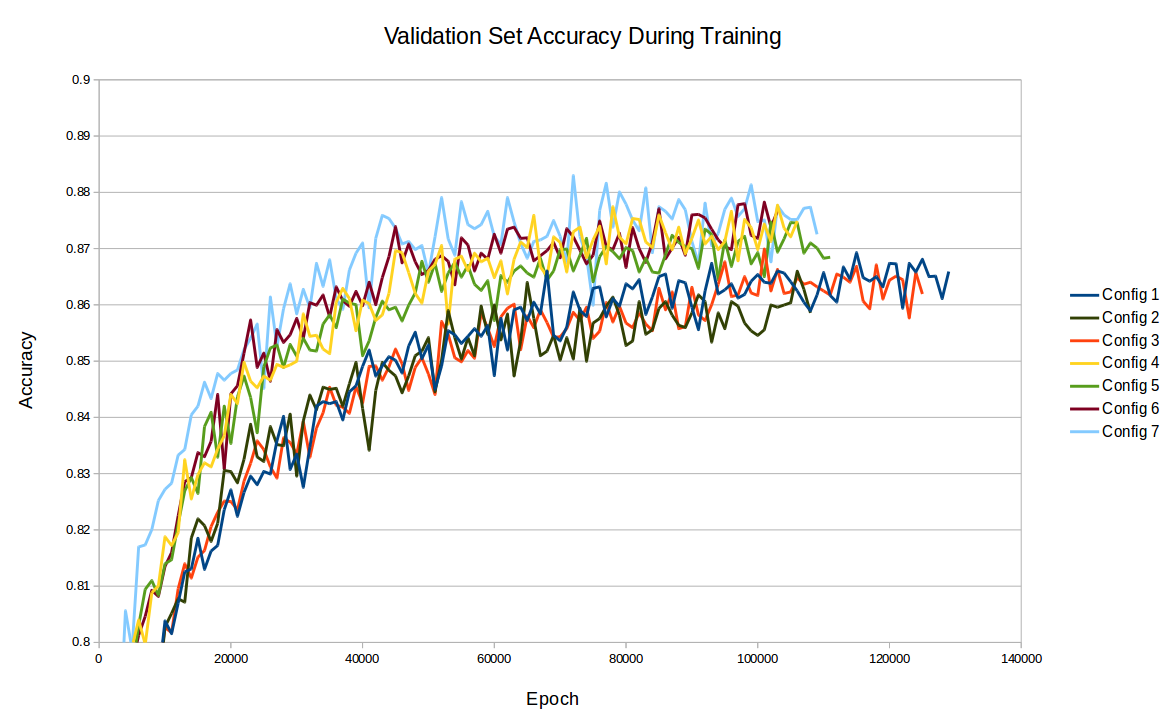
\includegraphics[width=1\textwidth]{plots/convplot}
\end{figure}

The final test set accuracies of the various configurations are shown in the table below. 

\begin{table}[h]
\centering
\caption{Test Set Accuracies}
\label{convtest}
\resizebox{\textwidth}{!}{
\begin{tabular}{|l|l|l|l|l|l|l|l|}
\hline
                  & Config 1 & Config 2 & Config 3 & Config 4 & Config 5 & Config 6 & Config 7 \\ \hline
Test Set Accuracy & 0.851    & 0.844    & 0.849    & 0.862    & 0.861    & 0.857    & 0.863    \\ \hline
\end{tabular}}
\end{table}


\subsection{Discussions}

There are numerous observations we can make from the results in Table \ref{convtest}. 

\subsubsection{Pooling}

Configuration 1 and Configuration 2 differ in the presence and absence of a max pooling layer that operates over non-overlapping 2x2 patches, respectively. In Configuration 1, there is one such layer after both the first and the second convolution layers, while in Configuration 2, there is only one such layer after the second convolution layer. 

Configuration 1 obtained 85.1\% accuracy on the test set, while Configuration 2 obtained 84.4\% accuracy. Moreover, the validation set error toward the end of the training also appears to be lower for Configuration 2. We can conclude that the pooling layer has an impact on our results. 

\subsubsection{}

\section{K-Nearest Neighbours}
K-Nearest Neighbours (K-NN) has traditionally performed very well in a variety of tasks so we will investigate the performance of K-NN in the SVHN domain. Using the raw pixel data ($32 x 32 x 3 = 3072$ dimensions) was too time intensive and so PCA was used to reduce the dimensionality to make the computations more feasible.  The PCA dimension space was determined through cross-validation as well as inspecting the eigenvector weights to determine the significance each eigenvector has for preserving the information contained in the dataset (see Section~\ref{knn_pca} for the direct analysis on top PCA dimensions).  Additionally, the number of neighbours to consider when determining the class for a new example (K hyper-parameter) was also determined using cross validation. \textbf{Finally, the tuned K and the PCA dimension hyper-parameters (PCA=3, K=7 chosen from Figure~\ref{fig:knn}) were trained with the "extra\_train" dataset to realize the optimal performance for K-NN in the SVHN domain given our data sets. The non-parametric classifier produced an accuracy of \%.(this takes too long..still want to do)}

\subsection{Determining PCA Dimension} \label{knn_pca}
The top 20 eigenvector weights were: [0.58293515, 0.05988745, 0.05289433, 0.04385749, 0.02023858, 0.01697088, 0.01630875, 0.01405416, 0.01276369, 0.01054048, 0.00940606, 0.00807162, 0.00638873, 0.00593508, 0.00566315, 0.00521857, 0.00484299, 0.00470581, 0.00434406, 0.00396934].  From inspecting this list, the first eigenvector is extremely influential in separating the classes and after the 4th eigenvector the difference in significance is negligible so we expected either negligible or no performance increase.  Therefore, we used PCA projected dimension spaces of $\{1, 2, 3, 4, 30\}$ to see the impact across the top eigenvectors as well as seeing if using additional, seemingly negligible, eigenvectors can have any impact.

\subsection{Determining K} \label{knn_k}
Given the problem is a ten-ary classification problem it seems natural that K should be fairly large, larger than a configuration for a binary classifier which ranges K from 1 to $\approx 15$ (in most domains).  Therefore cross validation is executed for all $K \in \{1, 7, 13, 19, 25, 31, 37, 43, 49, 55, 61\}$.  The choice of K is not a linear function because, although there are more classes, it should be that each class has a few classes that it may be similar to and others that are almost complete opposites.  For example, 1 will be similar to 7 and dissimilar others, 3 can be similar to 8 and 9, while 0 can be similar to 3, 8, and 9 by using common shapes and similar features like roundness and vertical and horizontal displacement.  Figure~\ref{fig:knn} illustrates that the optimal K was always less than $K=31$.

\subsection{Grayscale PCA Pixel Values}
Figure~\ref{fig:knn} shows the accuracy of using K-NN to classify SVHN using varying PCA dimension spaces and values for K. The accuracies range from $\approx 11.1\%$ to $\approx 11.8\%$; however, all are very low suggesting that looking at raw grayscale pixel values is not indicative of interpreting SVHNs (especially considering the extra redundancy in choosing extra PCA eigenvectors).  These results are only slightly better than random (10\%).  In conclusion, K-NN is clearly an extremely weak classifier for SVHN and is likely because of the nature of a colour/3-channel/high-dimensional input example coupled with a ten-class classification problem.  Even using grayscale inputs reduced the dimensions significantly, there is likely a lot of information that is lost (otherwise the accuracies would be much higher).  The use of PCA was successful in further reducing the grayscale image dimension as seen in Figure~\ref{fig:knn} which clearly shows that using the top 3 dimensions is sufficient and optimal (given our dataset).


\begin{figure}
\centering
	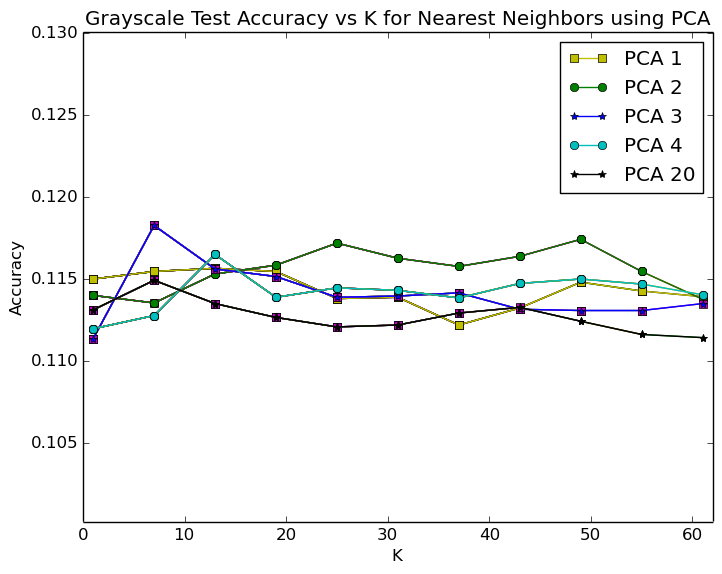
\includegraphics[width=0.8\linewidth]{./plots/knn/grayscale}
    	\caption{Performance of K-NN grayscale images projected into a Different Dimensional Spaces using PCA}
	\label{fig:knn}
\end{figure}

\subsubsection{Concluding Remarks}


\section{Conclusion}



\section*{Acknowledgments}

\section*{References}

\small{
\nocite{*}
\bibliographystyle{plainnat}
\bibliography{research}
}
\end{document}